\section{Wednesday 08/28/2024}

\begin{gather}
  max \text{ } {x_1 + x_2} \\
  s.t. \text{ } 3x_1 + x_2 \leq 3 \\
  x_1 \geq 0, x_2 \geq 0
\end{gather}

\begin{figure}[htbp]
  \centerline{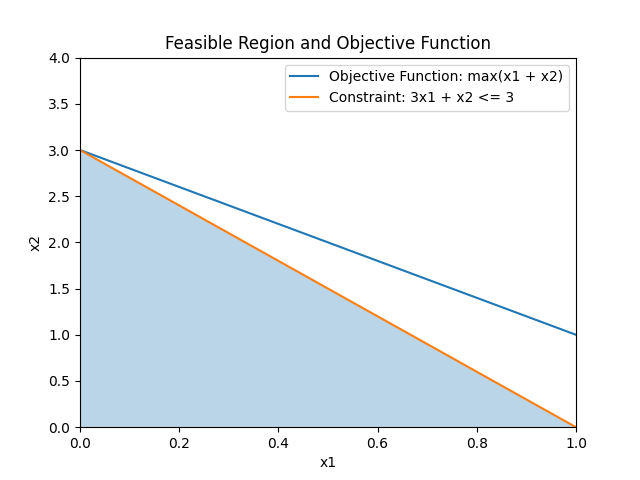
\includegraphics[width=0.8\textwidth]{images/08282024example.png}}
\end{figure}

$x^*$ is an extreme point if we cannot find $x_1, x_2 \in S, $ such that $x_1 \neq x_2 $ and
$x^* = \lambda x_1 + (1-\lambda)x_2$ for some $\lambda \in (0,1)$
\\
For an n-dimensional problem, there are n-many constraints that are active/binding and their coefficients are linearly independent. 
\\
Optimal solutions can be found that are not basic feasible solutions when constraints and objective functions lie on the same plane.
\\

\section{Friday 08/30/2024}
\subsection{Complexity Introduction}
Three elements for complexity analysis:
\begin{itemize}
  \item Model or problem formulation - The known part of a problem. Includes the formulation and problem descriptions.
  \item Oracle - The smallest computing unit, whose details inside can be ignored.
  \item Target outcome - When to stop
\end{itemize}

Two types of complexity:
\begin{itemize}
  \item Analytical complexity - The number of calls of the oracle which is necessary to solve a given problem formulation up to accuracy $\epsilon$
  \item Numerical complexity - The number of arithmetic operations which is necessary to solve a given problem formulation up to accracy $\epsilon$
\end{itemize}

\subsection{P, NP, NP-hard}
\framebox[\linewidth]{
    \begin{minipage}{\dimexpr\linewidth-2\fboxsep-2\fboxrule\relax}
        A \textbf{problem} is a function $F : I \to B$, where I is the set of instances encoded as strings of characters and B is the set of problem outputs.
    \end{minipage}
}

For example, linear programming in $\mathbb{R}^{mxn}$ is a problem where the instance parameters are $(m,n,A,c,b)$ and the output $B$ is the optimal solution found to the objective function.

Another example, making a decision takes in an instance $I$ and outputs a decision of yes or no.
\begin{equation}
  I = \textit{Problem-specific information parameters}, B \in (yes, no)
\end{equation}

